\section{Strömungsmechanik und CFD}
\label{sec:stroemungsmechanik_und_cfd}
In diesem Kapitel wird auf die grundlegende Theorie der
Strömungsmechanik und die CFD eingegangen, wobei nur die für die
Arbeit benötigte Theorie erklärt wird. Für weitere Theorie zur
Strömungsmechanik wird auf die Bücher \guillemotleft{}Strömungsmechanik\guillemotright{} von Hendrik
Kuhlmann~\cite{Backus67}, \guillemotleft{}Technische Fluidmechanik\guillemotright{} von Herbert Sigloch
\cite{Backus66} und \guillemotleft{}turbulence\guillemotright{} von P.A. Davidson
\cite{Bay00} verwiesen.

 Bei
den CFD-Aspekten werden die allgemeinen Einstellungen für die
durchgeführten Simulationen aufgelistet und erklärt, wobei speziell
die Randbedingungen und das Setup zur Sprache kommen.


\subsection{Theorie}
\label{subsec:theorie}
In diesem Abschnitt werden die wichtigsten Formeln und Begriffe dieser Arbeit genauer erklärt und beschrieben.

\paragraph{Strömungsarten} 
\label{para:stroemungsarten}
$\;$\\
In der Strömungslehre existieren zwei verschiedene Strömungsarten von Gasen und Flüssigkeiten:

        \begin{itemize}
        \item Laminare Strömung
        \item Turbulente Strömung
        \end{itemize}

Unter einer laminaren Strömung wird die Bewegung von Flüssigkeiten und Gasen verstanden, bei der sich die Schichten nicht miteinander vermischen. Dies ist in Abbildung \ref{fig:laminare_und_trubulente_stroemung} unter \flqq laminar Flow\frqq \, ersichtlich.
Die Bewegung von Fluiden, bei der Verwirbelungen auftreten, wird als turbulente Strömung bezeichnet. Dabei gibt es eine starke Vermischung der Schichten, wie in Abbildung \ref{fig:laminare_und_trubulente_stroemung} unter \flqq turbulent Flow\frqq \, zu erkennen ist.

        \begin{figure}[htb!]
        \begin{center}
        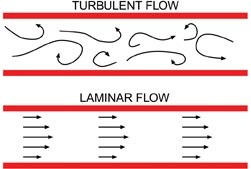
\includegraphics[width=5cm]{laminar_turbulent_stroemung}
        \caption{Beispiel für eine laminare und turbulente Strömung \cite{Backus66}}
        \label{fig:laminare_und_trubulente_stroemung}
        \end{center}
        \end{figure}

Strömungen, die in der Realität auftreten, bestehen aus den beiden
Strömungstypen. Damit eine Strömung turbulent wird, muss eine genügend
hohe Reynoldszahl vorhanden sein, welche bei der Strömung über eine
ebene Platte oder einem Flügelprofil bei ca. $3 \cdot 10^5$
liegt. Jedoch reisst beim Flügelprofil bei grossem Anstellwinkel die
Strömung früher ab. Überschreitet die Reynoldszahl diesen Wert, egal
ob über der ebenen Platte oder über dem Flügelprofil, so wird ein Übergang
zwischen laminar und turbulent stattfinden. Wie aus der Formel für die
Reynoldszahl (\ref{eq:reynoldszahl}) ersichtlich ist, wird der Wert
desto grösser, je grösser der Abstand zur Anfangskante ist. Zusätzlich hängt dieser Übergang von der Strömungsgeschwindigkeit $U_\infty$ ab. Ist dieser Wert in der Umgebung bereits hoch, kann es sein, dass die Strömung gleich nach Eintreffen über der Platte turbulent wird.


Um das Verständnis und die Rechnungen für diese Thematik zu erhalten, wurde das Buch \textit{Strömungsmechanik} von Hendrik Kuhlmann \cite[Kap. 7]{Backus67} und die Bachelorarbeit von Michael Schuler und Kyle Axel Elford \cite{Bay00} beigezogen. Nachfolgende Formeln werden alle aus den oben erwähnten Werken entnommen.\\


\paragraph{Reynoldszahl} 
\label{para:reynoldszahl_theorie}
$\;$ \\Die Reynoldszahl ist eine dimensionslose Kennzahl, die zur Beschreibung der Charakteristik einer Strömung  verwendet wird. Mit der Reynoldszahl lässt sich erkennen, ob eine laminare oder turbulente Strömung vorliegt. Sie berechnet sich aus dem Verhältnis zwischen Trägheitskraft und Reibungskraft in einer Strömung.

\begin{align}
\text{Re}= \dfrac{U \cdot L}{\nu} = \frac{\rho \cdot v \cdot x}{\eta}
\label{eq:reynoldszahl} 
\end{align}
\begin{center}
\begin{minipage}{0.5\linewidth}
$\text{Re} \dots \text{Reynoldszahl} \left[-\right]$ \\
$\rho \dots \text{Dichte} \left[\frac{kg}{m^3}\right]$ \\
$v \dots \text{Strömungsgeschwindigkeit} \left[\frac{m}{s}\right]$ \\
$x \dots \text{Abstand zum Profilanfang} \left[m\right]$ \\
$\eta \dots \text{dynamische Viskosität} \left[\frac{kg}{ms}\right]$ \\
\end{minipage}
\end{center}


\paragraph{Randschichtdicke}
\label{para:randschichtdicke_theorie}
$\;$ \\Eine Randschicht, oder auch Grenzschicht genannt, ist der Bereich einer Strömung, welcher in Wandnähe von der Reibung beeinflusst wird. Die Randschicht ist solange vorhanden, wie die Reibung einen Einfluss auf die Geschwindigkeit senkrecht zur Wand hat, was in Abbildung \ref{fig:grenzschichtdicke_theorie} die gestrichelte Linie darstellt. In der Randschicht sind grosse Geschwindigkeitsgradienten der Strömung vorhanden, denn unmittelbar an der Wand beträgt die Geschwindigkeit null. Mit (\ref{eq:randschichtdicke_laminar}) kann die Randschichtdicke für die laminare Strömung und mit (\ref{eq:randschichtdicke_turbulent}) für die turbulente Strömung berechnet werden. Die Randschichtdicke ist hier so definiert, dass die Geschwindigkeitskomponenten in X-Richtung 99\% von der Strömungsgeschwindigkeit am Einlass beträgt. Die Randschichtdicke ist in Abbildung \ref{fig:grenzschichtdicke_theorie} gestrichelt dargestellt.

\begin{align}
\delta_{lam} = 5.0 \cdot \sqrt{\dfrac{\nu \cdot x}{U_{\infty}}}
\label{eq:randschichtdicke_laminar} 
\end{align}
\begin{center}
\begin{minipage}{0.5\linewidth}
$\delta_{lam} \dots \text{Randschichtdicke laminar} \left[m\right]$
$\nu \dots \text{kinematische Viskosität} \left[\frac{m^2}{s}\right]$ \\
$x \dots \text{Abstand zum Profilanfang} \left[m\right]$ \\
$U_{\infty} \dots \text{Geschwindigkeit am Einlass} \left[\frac{m}{s}\right]$\\
\end{minipage}
\end{center}


\begin{align}
\delta_{turb} = 0.37 \cdot \left[\dfrac{\nu\left(x-x_0\right)^4}{U_{\infty}}\right]^\frac{1}{5}
\label{eq:randschichtdicke_turbulent}
\end{align}
\begin{center}
\begin{minipage}{0.5\linewidth}
$\delta_{turb} \dots \text{Randschichtdicke turbulent} \left[m\right]$
$\nu \dots \text{kinematische Viskosität} \left[\frac{m^2}{s}\right]$ \\
$x \dots \text{Abstand zum Plattenanfang} \left[m\right]$ \\
$x_0 \dots \text{fiktive Vorderkante der turbulenten Grenzschicht} \left[m\right]$
$U_{\infty} \dots \text{Geschwindigkeit am Einlass} \left[\frac{m}{s}\right]$\\
\end{minipage}
\end{center}

        \begin{figure}[htb!]
        \begin{center}
        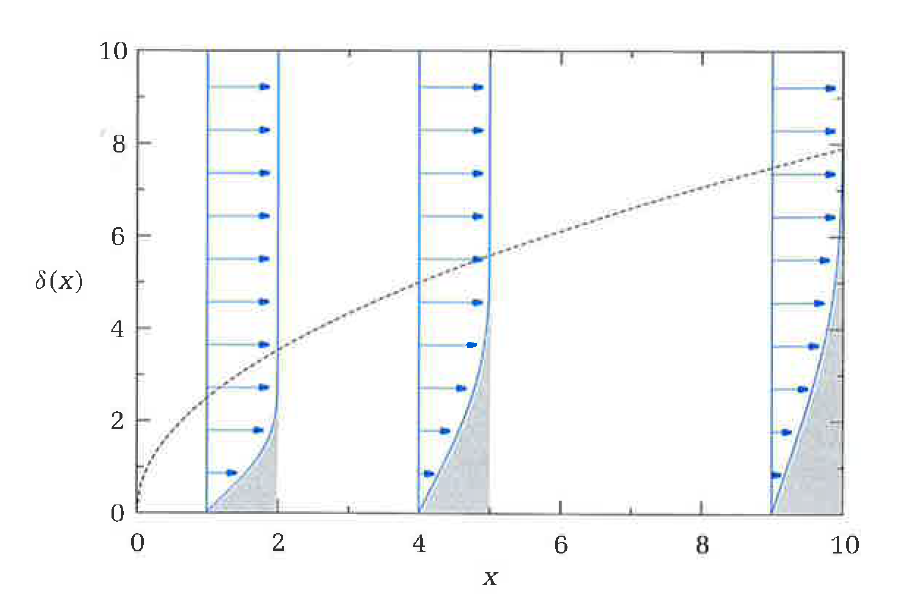
\includegraphics[width=0.5\textwidth]{grenzschichtdicke}
        \caption{Randschichtdicke (gestrichelt) als Funktion des Abstands \textit{x} zur Vorderkante einer angeströmten Platte. Die Geschwindigkeitsprofile sind blau angedeutet. Die Geschwindigkeitsdifferenz ist grau angedeutet. \cite[Kap.7, S. 223]{Backus66}}
        \label{fig:grenzschichtdicke_theorie}
        \end{center}
        \end{figure}

\newpage

\paragraph{Verdrängungsdicke}
\label{para:verdraengungsdicke_theorie}
$\;$ \\Eine weitere Möglichkeit, die Randschicht zu betrachten, bietet die Verdrängungsdicke. Mit dem  Anwachsen der Grenzschicht über den Verlauf der Oberfläche wird eine immer dickere Schicht des Fluids (Luft) verlangsamt.  Durch die geringere Geschwindigkeit in der Randschicht (graue Fläche in Abbildung \ref{fig:grenzschichtdicke_theorie}) wird der Volumenstrom in X-Richtung verkleinert. Um den gleichen Volumenstrom wie am Einlass beizubehalten, muss das Fluid nun seitlich ausweichen, was zu einer Geschwindigkeitskomponente in Y-Richtung führt. Dieses Ausweichen des Fluids wird als Verdrängungsdicke deklariert. Die Verdrängungsdicke ist physikalisch eindeutig definiert und kann mit (\ref{eq:verdraengungsdicke_laminar}) und (\ref{eq:verdraenungsdicke_turbulent}) für den laminaren und den turbulenten Fall berechnet werden.


\begin{align}
\delta_{lam,1}(x) &:=\frac{1}{U_{\infty}}\int^\infty_0\left(U_\infty-u\right)\text{d}y \nonumber\\
        &=\int^\infty_0\left(1-f'\right)\text{d}y\nonumber\\
        &=\sqrt{\frac{\nu x}{U_\infty}}\int^\infty_0\left(1-f'\right)\text{d}\eta\nonumber\\
        &=\sqrt{\frac{\nu x}{U_\infty}}\underbrace{\lim\limits_{\eta \rightarrow \infty}{\left[\eta-f(\eta)\right]}}_{\rightarrow 1.72}\nonumber\\
        &\simeq 1.72\sqrt{\frac{\nu x}{U_\infty}}\nonumber\\
        &\approx0.3444\cdot\delta(x)
\label{eq:verdraengungsdicke_laminar}
\end{align}
\begin{center}
\begin{minipage}{0.5\linewidth}
$\delta_{lam,1} \dots \text{Verdrängungsdicke laminar} \left[m\right]$
$U_{\infty} \dots \text{Geschwindigkeit am Einlass} \left[\frac{m}{s}\right]$\\
$u \dots \text{Geschwindigkeit in X-Richtung} \left[\frac{m}{s}\right]$\\
$f' \dots \text{Balsius-Gleichung =}\quad\frac{u}{U_{\infty}} \quad \left[-\right]$\\
$\nu \dots \text{kinematische Viskosität} \left[\frac{m^2}{s}\right]$ \\
$x \dots \text{Abstand zum Profilanfang} \left[m\right]$ \\
$\eta \dots \text{dynamische Viskosität} \left[\frac{kg}{ms}\right]$ \\
$\delta(x) \dots \text{Randschichtdicke an der Stelle x} \left[m\right]$\\
\end{minipage}
\end{center}

\begin{align}
\delta_{turb,1} &=\frac{1}{U_{\infty}}\int^\infty_0\left(U_\infty-\bar{u}\right)\text{d}y \nonumber\\
        &\approx \frac{\delta}{8}
\label{eq:verdraenungsdicke_turbulent}
\end{align}
\begin{center}
\begin{minipage}{0.5\linewidth}
$\delta_{turb,1} \dots \text{Verdrängungsdicke turbulent} \left[m\right]$
$U_{\infty} \dots \text{Geschwindigkeit am Einlass} \left[\frac{m}{s}\right]$\\
$\bar{u} \dots \text{mittlere Geschwindigkeit in X-Richtung} \left[\frac{m}{s}\right]$ \\
\end{minipage}
\end{center}
 

\paragraph{Definition von Auftrieb und Widerstand} 
\label{para:definition_von_auftrieb_und_wiederstand}
$\;$\\ 
Beim Umströmen eines Flügelprofils entstehen Kräfte auf der Flügeloberfläche. Diese Kräfte können äquivalent im sogenannten Druckpunkt zusammengefasst werden. Im Druckpunkt ist das wirkende Drehmoment null. Die Position des Druckpunktes eines Flügels ist vom Anstellwinkel abhängig. Damit die Berechnung vereinfacht werden kann, werden alle Kräfte auf den t/4-Punkt zusammengefasst. Durch den Abstand zwischen dem Druckpunkt und dem t/4-Punkt entsteht das Drehmoment. In Abbildung \ref{fig:definition_auftrieb_widerstand_moment} ist ein Flügelprofil dargestellt, bei dem die Kräfte auf den Flügel eingezeichnet sind. Daraus ist die resultierende Kraft R, welche aus dem Auftrieb A und dem Widerstand W besteht, ersichtlich. Der Auftrieb ist senkrecht zur Anströmrichtung, der Widerstand ist parallel zur Anströmrichtung. Zudem ergibt sich noch ein Drehmoment im t/4-Punkt, da der Druckpunkt ganz leicht abweicht. Der Auftrieb für das Flügelprofil entsteht  fast ausschliesslich aus den Druckunterschieden an der oberen und unteren Flügeloberfläche. Der Widerstand entsteht bei kleinen Anstellwinkeln hauptsächlich aus der Reibung zwischen dem Flügelprofil und der strömenden Luft. Bei grösseren Anstellwinkeln beginnt der Druckunterschied auch auf den Widerstand zu wirken. 


        \begin{figure}[htb!]
        \begin{center}
        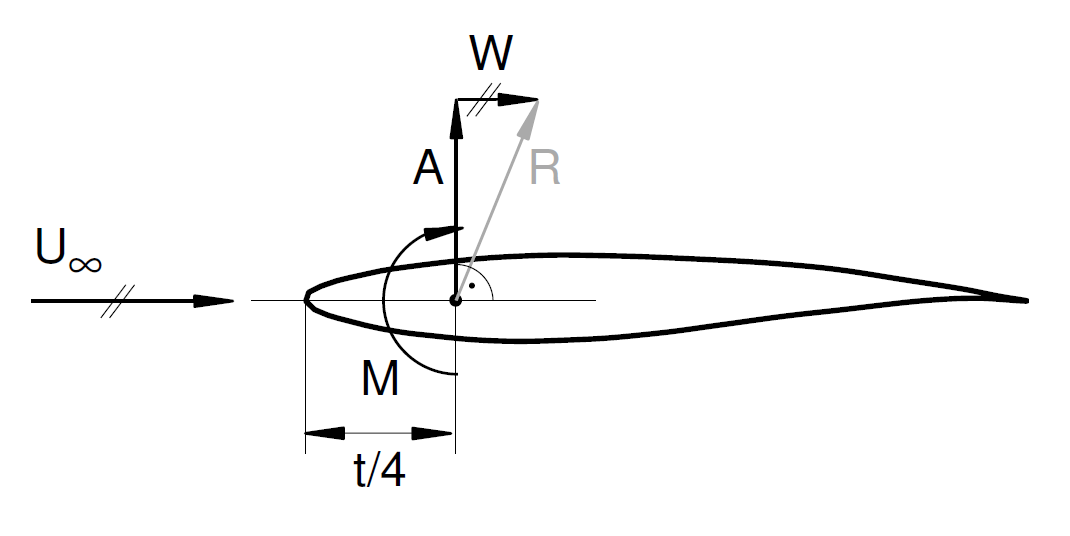
\includegraphics[width=8cm]{Definiton_Am_Fluegel}
        \caption{Definition von Auftriebskraft, Widerstandskraft und Drehmoment \cite{ESA98}}
        \label{fig:definition_auftrieb_widerstand_moment}
        \end{center}
        \end{figure}



In der Flugzeugindustrie werden anstelle des Drehmomentes und der Auftriebs- und Widerstandskräfte die dimensionslosen aerodynamischen Beiwerte verwendet. Mit diesen Beiwerten lassen sich Flügelprofile besser vergleichen als mit den Kräften. Ein wichtiger Faktor für die Beiwerte ist der Staudruck, welcher wie bei (\ref{eq:staudruck}) berechnet wird.\\
Mit (\ref{eq:auftreibsbeiwert}), (\ref{eq:widersteandsbeiwert}) und (\ref{eq:momentenbeiwert}) werden die verschiedenen Beiwerte berechnet. 

\begin{align}
q_\infty = \frac{\rho_\infty}{2}\cdot U\infty^2
\label{eq:staudruck}
\end{align}
\begin{align}
c_A = \frac{A}{q_\infty\cdot F} = \frac{A}{\frac{\rho_\infty}{2}\cdot U\infty^2\cdot F}
\label{eq:auftreibsbeiwert}
\end{align}
\begin{align}
c_W = \frac{W}{q_\infty\cdot F} = \frac{W}{\frac{\rho_\infty}{2}\cdot U\infty^2\cdot F}
\label{eq:widersteandsbeiwert}
\end{align}
\begin{align}
c_M = \frac{M}{q_\infty\cdot F} = \frac{M}{\frac{\rho_\infty}{2}\cdot U\infty^2\cdot F}
\label{eq:momentenbeiwert}
\end{align}

\begin{center}
\begin{minipage}{0.5\linewidth}
$q_\infty \dots \text{Staudruck} \left[\frac{kg}{s^2\cdot m}\right]$
$\rho_\infty \dots \text{Dichte} \left[\frac{kg}{m^3}\right]$ \\
$U\infty \dots \text{Umgebungsgeschwindigkeit} \left[\frac{m}{s}\right]$ \\
$c_A \dots \text{Auftriebsbeiwert} $\\
$F \dots \text{Flügelfläche} \left[m^2\right]$ \\
$c_W \dots \text{Widerstandsbeiwert} $\\
$c_M \dots \text{Momentbeiwert} $\\
\end{minipage}
\end{center}


\paragraph{Turbulenzen im Fluid} 
\label{para:turbulenzen_im_fluid}
$\;$\\
Turbulenz ist  in der Natur kein seltenes, sondern ein alltägliches Phänomen. Turbulenzen treten in allen Fluiden auf, jedoch ist es in der Realität schwierig, eine Turbulenz zu beschreiben und die Parameter dafür in ein Simulationsprogramm zu übergeben.


\subsection{CFD Aspekte}
\label{subsec:cfd_aspekte}
Folgend werden die Begriffe für die CFD-Simulation genauer erläutert und anschliessend die allgemeinen Einstellungen erklärt, welche bei allen Simulationen beibehalten werden, sofern nichts anderes erwähnt wird.

\paragraph{Y-Plus Wert} 
\label{para:y_plus_wert}
$\;$\\
Damit eine genaue Berechnung in der Wandnähe entsteht und die Ablösung
der Strömung oder der Widerstandsbeiwert richtig berechnet werden,
muss darauf geachtet werden, dass die erste Schicht der Vernetzung
genügend fein gewählt wird. Die Dicke der ersten Vernetzungsschicht
kann mit dem $y^+$ Wert untersucht werden und daraus die Schlüsse
gezogen werden, ob die Vernetzung senkrecht zur Wand oder zum Flügel
genügend fein ist. Mit der Vernetzung der Geometrie wird die Grösse
jedes einzelnen Elementes, welches bei der Simulation berechnet wird,
definiert. Das heisst je feiner die Vernetzung wird, desto mehr
Elemente entstehen und desto länger braucht das Programm, um die Simulation durchzuführen. Die Vernetzung wird in den einzelnen Kapiteln noch genauer erklärt.

Bei einer Simulation, bei der eine Ablösung stattfinden kann und der Widerstandsbeiwert berechnet werden soll, sollte darauf geachtet werden, dass der $y^+$ Wert ca. eins beträgt. Mit (\ref{eq:dicke_der_ersten_vernetzungsschicht}), welche aus der Bachelorarbeit von Michael Schuler und Kyle Axel Ford \cite{ESA98} entnommen wurde, kann die Dicke der ersten Vernetzungsschicht geschätzt werden.

\begin{align}
\Delta y &= d \, y^+ \sqrt{74}\, Re^{-\frac{13}{14}}
\label{eq:dicke_der_ersten_vernetzungsschicht}
\end{align}
\begin{center}
\begin{minipage}{0.5\linewidth}
$\Delta y \dots \text{Dicke der ersten Vernetzungsschicht} \left[m\right]$\\
$d \dots \text{spezifische Länge} \left[m\right]$ \\
$y^+ \dots \text{gewünschter y+ Wert} \left[-\right]$\\
$Re \dots \text{Reynoldszahl} \left[-\right]$ \\
\end{minipage}
\end{center}


\paragraph{Turbulenzmodelle} 
\label{para:turbulenzmodelle}
$\;$\\
Im Simulationstool ANSYS Workbench existieren verschiedene Turbulenzmodelle, welche für die Berechnungen eingestellt werden können. Dabei ist darauf zu achten, ob die Simulationen laminar bleiben oder ein Übergang in die turbulente Strömung erfolgen kann. Folgend werden die benutzen Modelle kurz erklärt.

\textbf{SST (Shear Stress Transport):} Das SST-Modell ist die
Kombination des $\kappa-\epsilon$ und\\ $\kappa-\omega$~Modells. Das SST Modell verhält sich in der Wandnähe
wie das $\kappa-\omega$ Modell und etwas abseits der Wandnähe
verhält es sich wie das $\kappa-\epsilon$ Modell. Dieses Modell wird
vor allem für die genauere Berechnung der Schubspannungen
verwendet. Zusätzlich wird für die Berechnung das
$\gamma-Re \theta$ Modell, welches in Ansys $\gamma-\theta$
Modell genannt wird, eingestellt. Die Einstellung dieses Modells
erlaubt es, den Übergang von der laminaren zur turbulenten Strömung zu
simulieren und zu untersuchen. So kann nachvollzogen werden, welche Wirkung die Vortexgeneratoren auf der Oberseite des Flügelprofils haben.

In ANSYS wird die Turbulenz mit den Einstellungen \guillemotleft{}Turbulence Intensity\guillemotright{} und \guillemotleft{}Turbulence length scale\guillemotright{} definiert, welche folgend genauer erklärt werden. Die \textbf{Turbulenz Intensität bzw. turbulence level} ist ein dimensionsloses Mass für die Intensität der Verwirbelung des Fluids. Bei der \textbf{turbulence length scale} handelt es sich um die Grösse der Verwirbelung am Inlet (Einlass). Je grösser die turbulence length scale ist, desto grösser ist die Verwirbelungsform. In  Tabelle \ref{tab:intensitaet} sind einige typische Werte eingetragen.

\begin{table}[htb!]
\begin{center}
    \begin{tabular}{lll}
    High   & 5\% - 20\% & Wärmetauscher, rotierende Maschinen \\
    Medium & 1\% - 5\%  & Rohrströmungen, Ventilation         \\
    Low    & < 1\%      & Luft um Autos, Flugzeug             \\

    \end{tabular}
    \end{center}
           \caption{Beispiele für Turbulenz Intensitäten \cite[S. 5]{Backus66}}
    \label{tab:intensitaet}
\end{table}

\newpage

\paragraph{Randbedingungen}
\label{para:randbedingungen_allgemein}
$\;$\\
Für die Simulationen wurden die vier folgenden Randbedingungseinstellungen vorgenommen, welche zusätzlich in Abbildung \ref{fig:randbedingungen_allgemein} dargestellt sind.\\

Der \textbf{Inlet} ist der Einlass des Fluids in die Simulationsumgebung und kann beliebig eingestellt werden. Beim Einlass werden die Einlassgeschwindigkeit, die Einlassrichtung und die Turbulenz eingestellt.
Auf die genauen Inleteinstellungen wird vor der Simulation eingegangen. \\

\textbf{Opening oben} und \textbf{Opening hinten} wird für den Übergang zur Umgebung verwendet. 
Bei einem Opening kann das Fluid sowohl hinein- als auch hinausströmen.
Bei den Opening-Einstellungen wurde ein Entrainment gewählt mit einem relativen Druck von \SI{0}{Pa}.
Bei den turbulenten Simulationen wurde zusätzlich beim Entrainment die Einstellung für die Turbulenz mit Zero Gradient gewählt. Durch diese Einstellung wird an beiden Openings keine Turbulenz vorgegeben. Dadurch werden die Resultate im interessanten Bereich kaum verfälscht. \\

Die \textbf{Wall} wurde verwendet, um die Oberfläche zu modellieren, die tatsächlich mit dem Fluid in Kontakt tritt. Es wird eine No Slip Wall verwendet, was bedeutet, dass das Fluid an der Oberfläche haftet und somit die Geschwindigkeit des Fluids direkt an der Oberfläche null beträgt. Durch den Geschwindigkeitsunterschied zwischen der Geschwindigkeit direkt an der Oberfläche und der Umgebung entsteht Reibung im Fluid. Aus der Reibung bildet sich die Randschicht über der Oberfläche.\\ 

Die \textbf{Symmetry} wird für die Ränder benutzt, die lediglich als Begrenzung zum restlichen Fluid dienen. 
Dabei gibt es kein Hinein- oder Hinausströmen des Fluids und die Geschwindigkeit senkrecht zur Randfläche ist null.\\ 


\begin{figure}[htb!]
	\begin{center}
	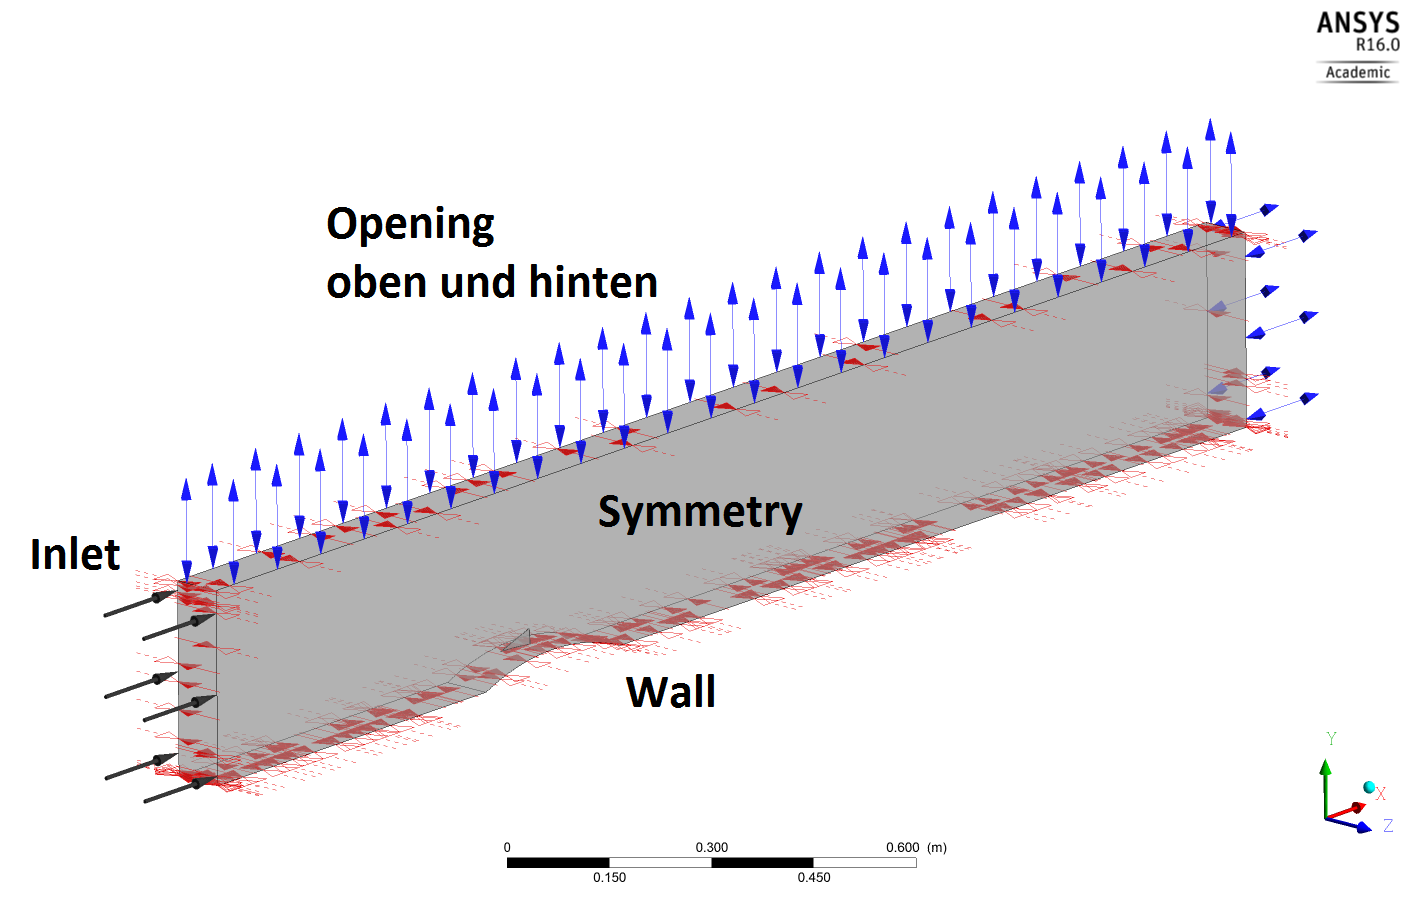
\includegraphics[width=0.8\textwidth]{randbedingungen_simulationsaufbau_denmark}
	\caption{Randbedingungen für die Simulation einer Wölbung mit einem Vortexgenerator}
	\label{fig:randbedingungen_allgemein}
	\end{center}
	\end{figure}

\newpage

\paragraph{Setup} 
\label{para:setup}
$\;$\\
Im folgenden Abschnitt werden die Simulationseinstellungen dargestellt, welche für alle Simulationen beibehalten werden, sofern nichts anderes erwähnt wird. Die Profilsimulationen werden als transiente Simulation durchgeführt mit einer maximalen Simulationszeit von \SI{2}{\second}. Als Zeitschritte werden zuerst 50x\SI{0.0001}{\second} und danach, bis zum Ende der Simulation, ein Zeitschritt von \SI{0.001}{\second} gewählt.\\
Die Simulationen werden isotherm bei \SI{25}{\celsius} durchgeführt und als Turbulenzmodell wird auf Shear Stress Transport mit $\gamma-\theta$ 
Modell eingestellt.\\
Die Fluideinstellungen für Luft sind wie folgt:

        \begin{itemize}
        \item Isothermische Simulation 
        \item Temperatur T             =       \SI{25}{[\celsius]}
        \item Referenzdruck p  =       1 $\left[atm\right]$
        \item Molare Masse M           =       0.02896 $\left[\frac{g}{mol}\right]$ 
        \item Dichte $\rho$                   =       1.185 $\left[\frac{kg}{m^3}\right]$ 
        \item Dynamische Viskosität $\eta$ = $18.31\cdot 10^-6 \left[\frac{kg}{m\, s}\right]$\\
        \end{itemize}


Beim Solver werden die folgenden Einstellungen gewählt:
\begin{itemize}
        \item Advection Scheme         = High Resolution 
        \item Transient Scheme         =       Second Order Backward Euler
        \item Timestep Initialization  =       Automatic
        \item Turbulence Numerics             =       High Resolution\\
        \\
        Convergence Control
        \item Min. Coeff. Loops               = 1
        \item Max. Coeff. Loops               = 15\\
        \\Convergence Criteria         
               
        \item Residual Type            = Max
        \item Residual Target          = 1e$^{-4}$ 
\end{itemize}

Bei transienten Rechnungen müssen unter Default Domain im Register Initialization bei den Einstellungen für die Turbulence folgende Einstellungen vorgenommen werden:

\begin{itemize}
 	\item $\text{Turbulence Option: Intensity and Length Scale mit:}$
	\item $\text{Fractional Intensity} = 0.00035 [-]$
	\item $\text{Eddy Length Scale} = 0.05 [m]$
\end{itemize}








